
\section{anti-anti-virus}

\begin{frame}{anti-anti-virus}
    \begin{itemize}
    \item defeating signatures:
    \vspace{.5cm}
    \item avoid things compilers/linkers never do
    \item make analysis harder
        \begin{itemize}
        \item takes longer to produce signatures
        \item takes longer to produce ``repair'' program
        \item may evade attempts to automate analysis
        \end{itemize}
    \item make changing viruses
        \begin{itemize}
        \item make any one signature less effective
        \end{itemize}
    \end{itemize}
\end{frame}





\begin{frame}{some terms}
    \begin{itemize}
    \item \myemph{armored} viruses
        \begin{itemize}
        \item viruses designed to make analysis harder
        \end{itemize}
    \item \myemph{metamorphic}/\myemph{polymorphic}/\myemph{oligomorphic} viruses
        \begin{itemize}
        \item viruses that change their code each time
        \item different terms --- different types of changes (later)
        \end{itemize}
    \end{itemize}
\end{frame}


\section{other obfuscation}
\subsection{why obfuscation, generally}
\begin{frame}{obfuscation, generally}
    \begin{itemize}
    \item malware often \textit{obfuscates} (obscures) its code
    \item several reasons for this
        \begin{itemize}
        \item prevent their from being signatures
        \item make analysis more difficult
        \item prevent others from modifying+copying
        \end{itemize}
    \vspace{.5cm}
    \item note: many of these technique sometimes employed by commercial software
        \begin{itemize}
        \item intended to prevent copying/reverse-engineering
        \end{itemize}
    \end{itemize}
\end{frame}


\section{Tigress and its transformations}
\begin{frame}{Tigress as example of obfuscation}
    \begin{itemize}
    \item Tigress --- researcher developer obfuscation tool
    \item \texttt{https://tigress.wtf}
    \item includes many \textit{transformations} typical of real-world obfuscation
        \begin{itemize}
        \item we'll talk about the ideas behind many of them
        \end{itemize}
    \vspace{.5cm}
    \item future assignment: modify code obfuscated with Tigress
    \end{itemize}
\end{frame}
\begin{frame}{example Tigress transformations}
    \begin{itemize}
    \item we'll look at some simple ones Tigress provides
    \item I'm showing you the pattern, \\ not the actual code Tigress generates
    \end{itemize}
\end{frame}

\begin{frame}[fragile,label=TigressMerge]{Tigress: provided transform: Merge}
\begin{lstlisting}[language=C++,style=smaller]
void foo(int a) { code for foo }
void bar(int a) { code for bar }

... foo(x) + bar(y) ...
\end{lstlisting}
\hrule
\begin{lstlisting}
void foo_bar(int s, int a) {
    if (s == 0) {
        code for foo
    } else {
        code for bar
    }
}

... foo_bar(0, x) + foo_bar(1, y) ...
\end{lstlisting}
\end{frame}

\begin{frame}[fragile,label=TigressSplit]{Tigress: provided transform: Split}
\begin{lstlisting}[language=C++,style=smaller]
void foo(int a, int b) {
    int x = ...;
    code for foo part 1
    code for foo part 2
}
\end{lstlisting}
\hrule
\begin{lstlisting}[language=C++,style=smaller]
void foo1(int *a, int *b, int *x) {
    code for foo part 1
}
void foo2(int *a, int *b, int *x) {
    code for foo part 2
}
void foo(int a, int b) {
    int x;
    foo1(&a,&b,&x); foo2(&a,&b,&x);
}
\end{lstlisting}
\end{frame}

\begin{frame}[fragile,label=TigressFlatten]{Tigress: example transform: Flatten}
\begin{lstlisting}[language=C++,style=smaller]
void foo() {
    A;
    if (X) {
        B;
    } else {
        C;
    }
    D;
}
\end{lstlisting}
\hrule
\begin{lstlisting}[language=C++,style=smaller]
void foo() {
    int s = 0;
    for (;;) {
        switch(s) {
        case 0: A; s = X ? 1 : 2; break;
        case 1: B; s = 3; break;
        case 2: C; s = 3; break;
        case 3: D; return;
        }
    }
}
\end{lstlisting}
\end{frame}

\begin{frame}{transformations so far?}
    \begin{itemize}
    \item all can be combined!
    \item annoying for analysis
    \item hard to do without unobfuscated code
        \begin{itemize}
        \item can't easily be redone/changed by self-replicating malware
        \end{itemize}
    \item probably more distinctive than original code for signatures
        \begin{itemize}
        \item (just match the transformed version since it won't change often)
        \end{itemize}
    \vspace{.5cm}
    \item next topic: transformations to avoid signatures
        \begin{itemize}
        \item (Tigress supports those, but not our primary examples)
        \end{itemize}
    \end{itemize}
\end{frame}


\section{obfuscation utility?}
\begin{frame}{obfuscation versus analysis}
    \begin{itemize}
    \item which of these does obfuscation seem most/least likely
        to hamper doing?
    \vspace{.5cm}
    \item A. determining what remote servers some malware contacts
    \item B. determining a password the malware requires to access extra functionality
    \item C. accessing extra functionality in the malware protected by a password
    \item D. determining whether the malware will behave differently based on the time
    \end{itemize}
\end{frame}


\section{packers}
\subsection{hashed data}
\begin{frame}[fragile,label=virusLibCall]{recall: library calls in viruses}
    \begin{itemize}
    \item viruses making library calls
        \begin{itemize}
        \item can't use normal dynamic linker stuff
        \end{itemize}
    \item common solution: search by name:
    \end{itemize}
\begin{lstlisting}[language=C++,style=smaller]
char *names[] = GetFunctionNamesFrom("kernel32.dll");
for (int i = 0; i < numFunctions; ++i) {
    if (strcmp(names[i], "GetFileAttributesA") == 0) {
        return functions[i];
    }
}
\end{lstlisting}
    \begin{itemize}
    \item problem: legit application code won't do this
    \item easy to look for string `GetFileAttributesA'
    \end{itemize}
\end{frame}

\begin{frame}[fragile,label=recallHideAPI]{searching for hashes}
\lstset{language=C,style=small}
\begin{lstlisting}
char *functionNames[] = GetFunctionsFromStandardLibrary();
/* 0xd7c9e758 = hash("GetFileAttributesA") */
unsigned hashOfString = 0xd7c9e758; 
for (int i = 0; i < num_functions; ++i) {
    unsigned functionHash = 0; 
    for (int j = 0; j < strlen(functionNames[i]); ++j) {
        functionHash = (functionHash * 7 +
                        functionNames[i][j]);
    }
    if (functionHash == hashOfString) {
        return functions[i];
    }
}
\end{lstlisting}
\end{frame}


\subsection{encrypted data}
\begin{frame}[fragile,label=encryptData]{encrypted(?) data}
\lstset{language=C,style=small}
\begin{lstlisting}
char obviousString[] =
    "Please open this 100%"
    " safe attachment";
char lessObviousString[] = 
    "oSZ^LZ\037POZQ\037KWVL\037\016\017"
    "\017\032\037L^YZ\037^KK^\\WRZQK";
for (int i = 0; i < sizeof(lessObviousString) - 1; ++i) {
    lessObviousString[i] =
        lessObviousString[i] ^ '?';
}
\end{lstlisting}
\end{frame}



\subsection{encrypted data and signatures}

\begin{frame}{encrypted data and signatures}
    \begin{itemize}
    \item get rid of some easy signatures
        \begin{itemize}
        \item especially if `key' changes or hashes used
        \end{itemize}
    \item but not enough:
        \begin{itemize}
        \item decryption code is very distinctive
        \end{itemize}
    \vspace{.5cm}
    \item<2-> can we do better with this ``encryption'' idea?
    \end{itemize}
\end{frame}



\subsection{encrypted code}

\begin{frame}[fragile,label=encrypted]{encrypted(?) viruses}
\lstset{language=C,style=small}
\begin{lstlisting}
char encrypted[] = "\x12\x45...";
char key[] = "...";
virusEntryPoint() {
    decrypt(encrypted, key);
    goto encrypted;
}
decrypt(char *buffer, char *key) {...}
\end{lstlisting}
\begin{itemize}
    \item choose a new key each time!
    \item not good encryption --- \myemph{key is there}
    \item sometimes mixed with \myemph{compression}
\end{itemize}
\end{frame}



\subsection{case study: Cascade}

\begin{frame}[fragile,label=cascade]{example: Cascade decrypter}
\lstset{
    style=small,
    language=myasm,
    moredelim={**[is][\btHL<2|handout:0>]{@hi2@}{@endhi@}},
    moredelim={**[is][\btHL<3|handout:0>]{@hi3@}{@endhi@}},
}
\begin{lstlisting}
    lea encrypted_code, %si
decrypt:
    mov $0x682, @hi3@%sp@endhi@ // length of body
    @hi2@xor %si, (%si)@endhi@
    @hi2@xor %sp, (%si)@endhi@
    inc %si
    dec @hi3@%sp@endhi@
    jnz decrypt
encrypted_code:
    ...
\end{lstlisting}
\imagecredit{Szor Listing 7.1}
\end{frame}




\section{exercise: handling decrypter}
\begin{frame}{exercise: some ideas for handling decrypters?}
    \begin{itemize}
    \item thinking of some anti-decrypter strategies for Cascade
    \item which of the following strategies most practical? least practical?
    \vspace{.5cm}
    \item A. matching patterns of decrypted malware code in memory while executables are running
    \item B. marking executables with too much random-looking data in them
    \item C. matching the decrypter in a normal signature scan
    \item D. trying every possible `key' for decryption on every executable and matching decrypted malware code against it
    \item E. detecting sequence of file operations Cascade makes instead of its code
    \end{itemize}
\end{frame}



\subsection{decrypter variations}
\usetikzlibrary{shapes.callouts}
\begin{frame}[fragile,label=decrypter]{decrypter}
    \begin{itemize}
    \item more variations:
        \begin{itemize}
        \item nested decrypters, different orders, etc.
        \end{itemize}
    \item still problem: \myemph{decrypter code is signature}
    \item \ldots but \myemph<2>{harder to distinguish\tikzmark{distinguish} different malware}
    \end{itemize}

    \begin{tikzpicture}[overlay,remember picture]
        \begin{visibleenv}<2>
        \node[my callout=distinguish,anchor=center] at ([yshift=-2cm]current page.center) {
            ``disinfection'' --- want to precisely identify malware
        };
        \end{visibleenv}
    \end{tikzpicture}
\end{frame}



\section{metamorphic, etc. idea}

\begin{frame}<1>[label=playMouse,fragile]{playing mouse}
    \begin{itemize}
    \item encrypted code? probably still have fast signature from decrypter
    \item goal: make signatures not work \textit{or} really slow
    \end{itemize}
\end{frame}




\section{oligomorphic viruses}
\againframe<2>{playMouse}
\usetikzlibrary{patterns}

\begin{frame}[fragile,label=olig]{oligomorphic virus/worm}
\begin{tikzpicture}
\draw[fill=yellow!30,very thick] (0, 0) rectangle ++(4, -1) node[midway] {code `decrypter'};
\draw[pattern=north west lines,pattern color=red,very thick] (0, -1) rectangle ++(4, -5);
    \node[anchor=south,fill=white] at (2, -5) {`encrypted' code};
    \draw[fill=white,thick,font=\small] (0.25, -2) rectangle ++ (3.5, -1) node[midway,align=center] {
        decrypter \\
        generator
    };
\node[anchor=north west,draw,very thick,font=\small] (decrypt gen code) at (5, -0.5) {
\begin{lstlisting}
int KEY = RAND();
write(MOV_OPCODE, ...);
...
for (int i = RAND(); i > 0; --i) 
    write(NOP_OPCODE);
...
write(XOR_OPCODE, KEY, ...);
...
\end{lstlisting}
};
\draw[thick,dashed] (3.75, -2) -- (decrypt gen code.north west);
\draw[thick,dashed] (3.75, -3) -- (decrypt gen code.south west);
\end{tikzpicture}
\end{frame}

\begin{frame}{producing changing malware}
    \begin{itemize}
    \item `encrypted' code can generate new decrypter
    \item not just {\tt nop}:
    \vspace{.5cm}
    \item switch between synonym instructions
        \begin{itemize}
        \item \texttt{add \$4, ...}, \texttt{sub \$-4, ...}
        \end{itemize}
    \item swap registers
    \item random instructions that manipulate `unused' registers
    \item \ldots
    \item template to generate a bunch of decrypters
        \begin{itemize}
        \item Szor calls such malware ``oligomorphic''
        \end{itemize}
    \end{itemize}
\end{frame}



\subsection{case study: W95/Memorial}

\begin{frame}[fragile,label=W95Memorial]{example: W95/Memorial}
\lstset{
    style=small,
    language=myasm,
    moredelim={**[is][\btHL<2|handout:0>]{@hi2@}{@endhi@}},
    moredelim={**[is][\btHL<3|handout:0>]{@hi3@}{@endhi@}},
}
\begin{tabular}{ll}
\begin{lstlisting}
  @hi2@mov $0x405000, %ebp@endhi@
  @hi2@mov $0x550, %ecx@endhi@
  lea 0x2e(%ebp), %esi
  add 0x29(%ebp), %ecx
  mov 0x2d(%ebp), %al

decrypt:
  nop
  nop
  xor %al, (%esi)
  inc %esi
  nop
  inc %al
  @hi3@dec %ecx@endhi@
  @hi3@jnz decrypt@endhi@
  ...
\end{lstlisting}
&
\begin{lstlisting}
  @hi2@mov $0x550, %ecx@endhi@
  @hi2@mov $0x13bc000, %ebp@endhi@
  lea 0x2e(%ebp), %esi
  add 0x29(%ebp), %ecx
  mov 0x2d(%ebp), %al

decrypt:
  nop
  nop
  xor %al, (%esi)
  inc %esi
  nop
  inc %al
  @hi3@loop decrypt@endhi@
  ...
  ...
\end{lstlisting}
\end{tabular}
    \imagecredit{Szor, Listsings 7.3 and 7.4}
\begin{tikzpicture}[overlay,remember picture]
    \begin{visibleenv}<2>
    \node[anchor=center,draw=red,ultra thick,fill=white] at (current page.center) {
        change instruction order; location of decryption key/etc.
    };
    \end{visibleenv}
    \begin{visibleenv}<3>
    \node[anchor=center,draw=red,ultra thick,fill=white] at (current page.center) {
        variable choices of loop instructions
    };
    \end{visibleenv}
    \begin{visibleenv}<4>
    \node[anchor=center,draw=red,ultra thick,fill=white] at (current page.center) {
        Szor: ``96 different decryptor patterns''
    };
    \end{visibleenv}
\end{tikzpicture}
\end{frame}




\section{polymorphic viruses}

\begin{frame}{more advanced changes?}
    \begin{itemize}
    \item Szor calls W95/Memorial \myemph{oligomoprhic}
        \begin{itemize}
        \item ``encrypted'' code
        \item plus \myemph{small} changes to decrypter
        \end{itemize}
    \item What about doing more changes to decrypter?
        \begin{itemize}
        \item many, many variations
        \end{itemize}
    \item Szor calls doing this \myemph{polymorphic}
    \item polymorphic example: 1260
    \end{itemize}
\end{frame}



\subsection{case study: 1260}

\begin{frame}[fragile,label=v1260]{example: 1260 (virus)}
\lstset{
    style=small,
    language=myasm,
    moredelim={**[is][\btHL<2-3|handout:0>]{@hi2@}{@endhi@}},
    moredelim={**[is][\btHL<4-5|handout:0>]{@hi3@}{@endhi@}},
}
% FIXME: adapt Listing 7.5
\begin{tabular}{ll}
\begin{lstlisting}
    @hi2@inc %si@endhi@
    mov @hi3@$0x0e9b@endhi@, %ax
    @hi2@clc@endhi@
    mov $0x12a, %di
    @hi2@nop@endhi@
    mov $0x571, %cx
decrypt:
    xor %cx, (%di)
    @hi2@sub %dx, %bx@endhi@
    @hi2@sub %cx, %bx@endhi@
    @hi2@sub %ax, %bx@endhi@
    @hi2@nop@endhi@
    @hi2@xor %cx, %dx@endhi@
    xor %ax, (%di)
    ...
\end{lstlisting}
&
\begin{lstlisting}
    mov @hi3@$0x0a43@endhi@, %ax
    @hi2@nop@endhi@
    mov $0x15a, %di
    @hi2@sub %dx, %bx@endhi@
    @hi2@sub %cx, %bx@endhi@
    mov $0x571, %cx
    @hi2@clc@endhi@
decrypt:
    xor %cx, (%di)
    @hi2@xor %cx, %dx@endhi@
    @hi2@sub %cx, %bx@endhi@
    @hi2@nop@endhi@
    @hi2@xor %cx, %bx@endhi@
    xor %ax, (%di)
    ...
\end{lstlisting}
\end{tabular}
\imagecredit{adapted from Szor, Listing 7.5}
\begin{tikzpicture}[overlay,remember picture]
    \begin{visibleenv}<3>
    \node[anchor=center,draw=red,ultra thick,fill=white] at (current page.center) {
        do-nothing instructions
    };
    \end{visibleenv}

    \begin{visibleenv}<5>
    \node[anchor=center,draw=red,ultra thick,fill=white] at (current page.center) {
        different decryption ``key''
    };
    \end{visibleenv}
\end{tikzpicture}
\end{frame}



\subsection{more generic mutation}

\begin{frame}[fragile,label=mutationEngine]{`mutation engine'}
\begin{lstlisting}[language=C++,style=small]
CopyDecrypter(original_code, new_code) {
    for (each instruction in original_code) {
        new_code += RandomNumberOfNops();
        new_code += PossiblyChooseVariant(instruction)
    }
}
\end{lstlisting}
\end{frame}



\section{terminology: packers}
\begin{frame}{terminology: packers}
    \begin{itemize}
    \item programs that decode and run code at runtime called \textit{packers}
    \item packages exist to do this for non-malware reasons
    \item example motivation: compression
    \end{itemize}
\end{frame}


\section{anti-packer strategies} % FIXME: move earlier?
\subsection{generic anti-packers}

\begin{frame}<1>[label=findingPackers]{handling packers}
    \begin{itemize}
    \item easiest way to decrypt self-decrypting code --- run it!
    \item solution: \myemph<1>{virtual machine/emulator/debugger} in antivirus software
    \end{itemize}
\end{frame}

\begin{frame}{handling packers with debugger/emulator/VM}
    \begin{itemize}
    \item run program in debugger/emulator/VM for a while
        \begin{itemize}
        \item one heuristic: until it jumps to written data
        \end{itemize}
    \item example implementation: unipacker (\texttt{https://github.com/unipacker/unipacker})
    \vspace{.5cm}
    \item then scan memory for decrypted machine code
    \item or obtain trace of instructions run
    \vspace{.5cm}
    \end{itemize}
\end{frame}

\begin{frame}{unneeded steps}
    \begin{itemize}
    \item understanding the ``encryption'' algorithm
        \begin{itemize}
        \item more complex encryption algorithm won't help
        \end{itemize}
    \item extracting the key and encrypted data
        \begin{itemize}
        \item making key less obvious won't help
        \end{itemize}
    \end{itemize}
\end{frame}


\begin{frame}[fragile,label=instrTraces1]{using instruction traces (1)}
\begin{itemize}
\item instruction traces are huge\ldots
\end{itemize}
\begin{lstlisting}
0x10: add %rax, %rbx
0x12: mov 0x140(%rbx), %rsi
0x14: mov %rsi, 0x150(%rbx)
0x16: jle 0x10
0x10: add %rax, %rbx        /* duplicate of before */
0x12: mov 0x140(%rbx), %rsi
0x14: mov %rsi, 0x150(%rbx)
0x16: jle 0x10
0x18: mov $10, %rcx
...
\end{lstlisting}
\begin{itemize}
\item but can simplify: e.g. remove duplicates (loops)
\end{itemize}
\end{frame}

\begin{frame}[fragile,label=instrTraces2]{using instruction traces (2)}
\begin{itemize}
\item elegant way to analyze `tricky' techniques
\item self-modifying code:
\end{itemize}
\begin{lstlisting}
    0x10: add %rax, %rbx
    0x12: mov 0x140, %rax
    0x14: mov %rsp, 0x0C
        /* modifies code we will execute */
    0x16: jle 0x10
    0x10: sub %rcx, %rdx
    0x12: ...
\end{lstlisting}
\begin{itemize}
\item multiple layers of `decrypters'/code generation
\item \ldots
\end{itemize}
\end{frame}




\section{emulators}
\subsection{exámple: unicorn}

\begin{frame}{unicorn as tool}
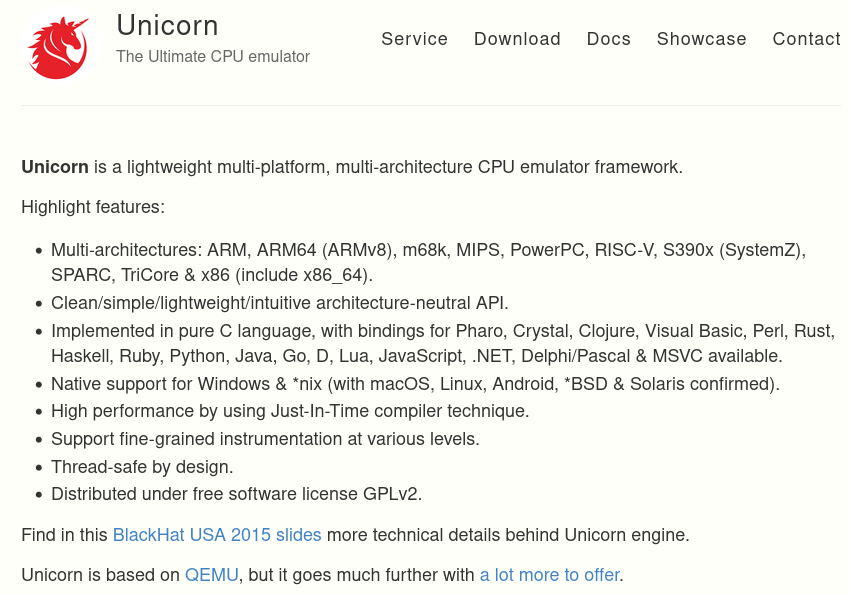
\includegraphics[width=\textwidth]{../antianti/unicorn-page}
\end{frame}

\begin{frame}[fragile]{unicorn example (1)}
\begin{Verbatim}[fontsize=\small]
$ cat test.s
    mov $10000, %edi
    imul $2, %rdi, %rdi
$ gcc -c test.s; objcopy -j .text test.o -O binary test.bin
\end{Verbatim}
\begin{Verbatim}[fontsize=\small]
code = Path('test.bin').read_bytes()
uc = Uc(UC_ARCH_X86, UC_MODE_64)
uc.mem_map(0x10000, 1024 * 1024)
uc.mem_write(0x10000, code)
uc.emu_start(0x10000, 0x10000 + len(code))
print("RDI",uc.reg_read(UC_X86_REG_RDI))
\end{Verbatim}
\hrule
\texttt{RDI 20000}
\end{frame}

\begin{frame}[fragile]{unicorn example (2)}
\begin{Verbatim}[fontsize=\small]
...
uc.hook_add(UC_HOOK_CODE, hook_code_func)
def hook_code_func(uc, addr, size, user_data):
    print(f"{addr:x} ({size} byte instruction): "
          f"{codecs.encode(uc.mem_read(addr, size), 'hex').decode()}")
uc.emu_start(0x10000, 0x10000 + len(code))
\end{Verbatim}
\hrule
\begin{Verbatim}[fontsize=\small]
10000 (5 byte instruction): bf10270000
10005 (4 byte instruction): 486bff02
\end{Verbatim}
\end{frame}


\begin{frame}[fragile]{unipacker psuedocode}
\begin{Verbatim}[fontsize=\small]
data, size = parse_executable()
uc.mem_map(BASE_ADDR, size)
uc.mem_write(BASE_ADDR, data)
for dll in get_executable_libraries():
    uc.mem_map(dll['addr'], dll['size'])
    uc.mem_write(dll['addr'], dll['data'])
...
uc.hook_add(UC_HOOK_CODE, before_execute)
uc.emu_start(...)

def before_execute(...): # called before each instruction
    ...
    if address in MODIFIED_SECTION:
        dump_memory_now()
\end{Verbatim}
\end{frame}



\subsection{aside: instruction traces}
\begin{frame}{traces instead of unpacked code}
    \begin{itemize}
    \item instead of matching signatures on code at rest
    \item can match signature on \textit{trace} of executed instructions
    \end{itemize}
\end{frame}

\begin{frame}[fragile,label=instrTraces1]{using instruction traces (1)}
\begin{itemize}
\item instruction traces are huge\ldots
\end{itemize}
\begin{lstlisting}
0x10: add %rax, %rbx
0x12: mov 0x140(%rbx), %rsi
0x14: mov %rsi, 0x150(%rbx)
0x16: jle 0x10
0x10: add %rax, %rbx        /* duplicate of before */
0x12: mov 0x140(%rbx), %rsi
0x14: mov %rsi, 0x150(%rbx)
0x16: jle 0x10
0x18: mov $10, %rcx
...
\end{lstlisting}
\begin{itemize}
\item but can simplify: e.g. remove duplicates (loops)
\end{itemize}
\end{frame}

\begin{frame}[fragile,label=instrTraces2]{using instruction traces (2)}
\begin{itemize}
\item elegant way to analyze `tricky' techniques
\item self-modifying code:
\end{itemize}
\begin{lstlisting}
    0x10: add %rax, %rbx
    0x12: mov 0x140, %rax
    0x14: mov %rsp, 0x0C
        /* modifies code we will execute */
    0x16: jle 0x10
    0x10: sub %rcx, %rdx
    0x12: ...
\end{lstlisting}
\begin{itemize}
\item multiple layers of `decrypters'/code generation
\item \ldots
\end{itemize}
\end{frame}



\section{packer issues}
\subsection{packers and W xor X/DEP}

\begin{frame}[fragile]{stopping packers}
    \begin{itemize}
    \item it's \myemph<2>{unusual} to jump to code you wrote
    \item modern OSs/compilers: memory not writeable and executable
    \end{itemize}
\vspace{.5cm}
\begin{visibleenv}<2->
\begin{Verbatim}[fontsize=\fontsize{10}{11}\selectfont,commandchars=\\\{\}]
LOAD off    0x00000000 vaddr 0x00000000 paddr 0x00000000 align 2**12
     filesz 0x00003458 memsz 0x00003458 flags \myemph{r--}
LOAD off    0x00004000 vaddr 0x00004000 paddr 0x00004000 align 2**12
     filesz 0x00013091 memsz 0x00013091 flags \myemph{r-x}
LOAD off    0x00018000 vaddr 0x00018000 paddr 0x00018000 align 2**12
     filesz 0x00007458 memsz 0x00007458 flags \myemph{r--}
LOAD off    0x0001ffd0 vaddr 0x00020fd0 paddr 0x00020fd0 align 2**12
     filesz 0x000012a8 memsz 0x00002570 flags \myemph{rw-}
\end{Verbatim}
\end{visibleenv}
\end{frame}

\begin{frame}{diversion: DEP/{\tt W\textasciicircum X}}
    \begin{itemize}
    \item memory executable or writeable --- but not both
    \item exists for \myemph{exploits} (later in course), not packers
    \item requires hardware support to be fast (\myemph{early 2000s+})
    \item various names for this feature:
        \begin{itemize}
        \item Data Execution Prevention (DEP) (Windows)
        \item {\tt W\textasciicircum X} (``write XOR execute'')
        \item NX/XD/XN bit  (underlying hardware support)
            \begin{itemize}
            \item (No Execute/eXecute Disable/eXecute Never)
            \end{itemize}
        \end{itemize}
    \item usually \myemph{special system call} to switch modes
        \begin{itemize}
        \item Linux: \texttt{mprotect}
        \end{itemize}
    \end{itemize}
\end{frame}

\begin{frame}{unusual, but\ldots}
    \begin{itemize}
    \item binary translation
        \begin{itemize}
        \item convert machine code to new machine code at runtime
        \end{itemize}
    \item Java virtual machine, JavaScript implementations
        \begin{itemize}
        \item ``just-in-time'' compilers
        \end{itemize}
    \item dynamic linkers
        \begin{itemize}
        \item load new code from a file --- same as writing code?
        \end{itemize}
    \item those packed commercial programs
    \vspace{.5cm}
    \item programs need to \myemph{explicitly} ask for write+exec
    \end{itemize}
\end{frame}


\subsection{exercise: limitations of generic anti-packer}
\begin{frame}{exercise: generic detection limits?}
    \begin{itemize}
    \item consider strategy of running executable in virtual machine, \\
          waiting until it jumps to code it wrote out \\
          then matching patterns against code it's about to run
    \item which of these would cause problems with this technique?
    \item which are easiest/hardest to workaround?
    \vspace{.5cm}
    \begin{itemize}
    \item A. code decrypter and malicious code run at program exit, not startup
    \item B. code decrypter and malicious code run when user clicks button in program, not at startup
    \item C. code decrypter allocates random address to write decrypted code to
    \item D. code decrypter exits (without running malicious code) if processor seems too slow
    \item E. code decrypter decrypts another code decrypter
    \end{itemize}
    \end{itemize}
\end{frame}


\section{metamorphic viruses}
     %FIXME: not very clear

\begin{frame}{changing bodies}
    \begin{itemize}
    \item ``decrypting'' a malware body gives body for ``signature''
        \begin{itemize}
        \item ``just'' need to run decrypter
        \end{itemize}
    \item how about avoiding static signatures entirely 
        \begin{itemize}
        \item despite being self-replicating
        \end{itemize}
    \item called \myemph{metamorphic}
        \begin{itemize}
        \item versus \myemph{polymorphic} --- only change ``decrypter''
        \end{itemize}
    \end{itemize}
\end{frame}



\subsection{example: changing bodies}

\begin{frame}[fragile,label=regSwap]{example: changing bodies}
\lstset{language=myasm,style=smaller}
\begin{tabular}{ll}
\begin{lstlisting}
pop %edx
mov $0x4h, %edi
mov %ebp, %esi
mov $0xC, %eax
add $0x88, %edx
mov (%edx), %ebx
mov %ebx, 0x1118(%esi,%eax,4)
\end{lstlisting}
&
\begin{lstlisting}
pop %eax
mov $0x4h, %ebx
mov %ebp, %esi
mov $0xC, %edi
add $0x88, %eax
mov (%eax), %esi
mov %esi, 0x1118(%esi,%eax,4)
\end{lstlisting}
\end{tabular}
\begin{itemize}
\item code above: after decryption
\item \myemph{every instruction} changes
\item still has good signatures
    \begin{itemize}
    \item with \myemph{alternatives} for each possible register selection
    \end{itemize}
\item but harder to write/slower to match
\end{itemize}
\end{frame}




\subsection{case study: Evol}
\usetikzlibrary{arrows.meta,positioning,matrix,calc,patterns}
\begin{frame}<1>[fragile,label=caseEvol]{case study: Evol}
    \begin{itemize}
    \item via Lakhatia et al, ``Are metamorphic viruses really invincible?'', Virus Bulletin, Jan 2005.
    \item ``\myemph{mutation engine}''
        \begin{itemize}
        \item run as part of propagating the virus
        \end{itemize}
    \end{itemize}
    \begin{tikzpicture}
        \tikzset{
            every node/.style={font=\small,align=center},
            hiOn/.style={alt=<#1>{red,ultra thick}{}},
        }
        \path node[draw,hiOn=2] (disasm) {disassemble} -- ++(2.5cm,0) node (lens) {instr. \\ lengths} -- ++(2cm,0) node[draw,hiOn=3] (xform) {transform}
              -- ++(2cm,0) node[draw,hiOn=4] (reloc) {relocate};
        \node (origCode) at ([xshift=-2cm,yshift=1cm]disasm.north) {code};
        \node (finalCode) at ([xshift=2cm,yshift=-1cm]reloc.south) {code};
        \begin{scope}[thick,-Latex]
        \draw (origCode) |- (disasm);
        \draw (disasm) -- (lens);
        \draw (lens) -- (xform);
        \draw (xform) -- (reloc);
        \end{scope}
    \end{tikzpicture}
\end{frame}

\againframe<2>{caseEvol}

\begin{frame}{Evol instruction lengths}
    \begin{itemize}
    \item sounds really complicated?
    \item virus only handles instructions it has:
        \begin{itemize}
        \item about 61 opcodes, 32 of them identified by first four bits
            \begin{itemize}
            \item e.g. opcode {\tt 0x7\textit{x}} -- conditional jump
            \end{itemize}
        \end{itemize}
    \item no prefixes, no floating point
    \item only {\tt \%reg} or {\tt \$constant} or {\tt offset(\%reg)}
    \end{itemize}
\end{frame}

\againframe<3>{caseEvol}

\begin{frame}[fragile,label=evolXform]{Evol transformations}
\lstset{language=myasm,style=small}
    \begin{itemize}
    \item some stuff left alone
    \item static or random one of $N$ transformations
    \item example:
    \end{itemize}
\begin{tikzpicture}
\tikzset{
    every node/.style={font=\small,align=center}
}
\node[draw] (movebpEight) {
\begin{lstlisting}
mov %eax, 8(%ebp)
\end{lstlisting}
};

\node[draw,right=2cm of movebpEight] (movebpExpand) {
\begin{lstlisting}
push %ecx
mov %ebp, %ecx
add $0x12, %ecx
mov %eax, -0xa(%ecx)
pop %ecx
\end{lstlisting}
};
\node[anchor=north east] at ([yshift=-.25cm]movebpExpand.south east) {
    uses more stack space --- save temporary \\
    code gets bigger each time
};
\end{tikzpicture}
\imagecredit{Lakhotia et al., ``Are metamorphic viruses really invincible?'', Virus Bulletin, Jan 2005}
\end{frame}

\againframe<4>{caseEvol}



\subsection{handling relocation with mutation}
\begin{frame}{mutation with relocation}
    \begin{itemize}
    \item problem: mutations mess up jumps/calls
        \begin{itemize}
        \item change were targets of jumps/calls are
        \end{itemize}
    \item table mapping old to new locations
        \begin{itemize}
        \item list of number of bytes generated by each transformation
        \end{itemize}
    \item list of locations references in original
        \begin{itemize}
        \item record relative offset in jump
        \item record absolute offset in original
        \end{itemize}
    \end{itemize}
\end{frame}

\begin{frame}[fragile,label=relocEx]{relocation example}
\lstset{language=myasm,style=small}
\begin{tikzpicture}
\node (code) {
\begin{lstlisting}
    mov ...
    mov ...
decrypt:
    xor %rax, (%rbx)
    inc %rbx
    dec %rcx
    jne decrypt
\end{lstlisting}
};
\matrix[tight matrix,nodes={font=\small},anchor=north west,
    nodes={font=\tt,text width=2cm,text depth=.1mm,minimum height=.4cm},
    row 1/.style={nodes={font=\small\bfseries,minimum height=1cm}},
    column 1/.style={text=blue!60!black,nodes={text width=1.75cm}},
    column 2/.style={text=green!60!black},
    column 3/.style={nodes={text width=1.5cm,font=\small\tt}},
] (lensTable) at ([xshift=1cm]code.north east) {
    orig. len \& new len \& instr \\
    5 \& 10 \& mov1 \\
    2 \& 3 \& mov2 \\
    2 \& 7 \& xor1 \\
    1 \& 1 \& inc1 \\
    1 \& 5 \& dec1 \\
    3 \& 3 \& jne1 \\
};
\matrix[tight matrix,nodes={font=\fontsize{9}{10}\selectfont,minimum height=1.2cm},anchor=north west,
    nodes={font=\tt,text width=4cm},
    row 1/.style={nodes={font=\small\bfseries,minimum height=1cm}},
    column 2/.style={text=blue!60!black},
    column 1/.style={text=green!60!black},
    column 3/.style={text=green!60!black},
] (relocTable) at ([yshift=-.5cm,xshift=-6.5cm]lensTable.south west) {
    address loc \& orig. target \& new target \\
    $10+3+7+1+5+1$ (jne1+1) \& xor1 ($5+2$)\& xor1 ($10+3$)\\ 
};
\end{tikzpicture}
\end{frame}



\subsection{fancy mutation engines}

\begin{frame}{mutation engines}
    \begin{itemize}
    \item tools for writing polymorphic viruses
    \item best: \myemph{no} constant bytes, \myemph{no} ``no-op'' instructions
    \item tedious work to build state-machine-based detector
        \begin{itemize}
        \item ((almost) a regular expression to match it)
        \item apparently done manually
        \item automatable?
        \end{itemize}
    \item (but probably can\ldots)
    \item pattern: used until reliably detected
    \end{itemize}
\end{frame}

\begin{frame}[fragile,label=fancyMut]{fancier mutation}
\begin{lstlisting}[style=script]
Mutate(original_machine_code, new_machine_code) {
    for (instruction in original_code) {
        new_machine_code += ChooseNewCodeFor(instruction)
    }
    FixupJumpsIn(new_machine_code);
}
\end{lstlisting}
    \begin{itemize}
    \item can do mutation on \myemph{generic machine code}
    \vspace{.5cm}
    \item ``just'' need full disassembler
    \item identify both \myemph{instruction lengths} and \myemph{addresses}
    \item hope machine code not written to rely on machine code sizes, etc.
    \item hope to identify \myemph{tables of function pointers}, etc.
    \end{itemize}
\end{frame}

\begin{frame}{fancier mutation}
    \begin{itemize}
    \item also an infection technique
        \begin{itemize}
        \item no ``cavity'' needed --- create one
        \end{itemize}
    \item obviously tricky to implement
        \begin{itemize}
        \item need to fix all executable headers
        \item what if you misparse assembly?
        \item what if you miss a function pointer?
        \end{itemize}
    \item example: Simile virus
    \end{itemize}
\end{frame}




\section{anti-virtualization strategies}
\subsection{basic issues}
\begin{frame}{antivirtualization}
    \begin{itemize}
    \item a lot of malware tries to behave different in a VM
    \vspace{.5cm}
    \item why?
        \begin{itemize}
        \item used by antivirus software to handle packers
        \item used to analyze malware
        \item \ldots
        \end{itemize}
    \end{itemize}
\end{frame}


\begin{frame}<1>[label=antivirtIndex]{antivirtualization techniques}
    \begin{itemize}
    \item \myemph<2-3>{query virtual devices}
        \begin{itemize}
        \item<3-> solution: mirror devices of some real machine
        \end{itemize}
    \item \myemph<4-5>{time operations that are slower in VM/emulation}
        \begin{itemize}
        \item<5-> solution: virtual clock
        \end{itemize}
    \item \myemph<6-7>{use operations not supported by VM}
        \begin{itemize}
        \item<7-> solution: support everything
        \end{itemize}
    \end{itemize}
\end{frame}

\againframe<2>{antivirtIndex}

\begin{frame}{virtual devices}
    \begin{itemize}
    \item VirtualBox device drivers?
    \item VMware-brand ethernet device?
    \item \ldots
    \end{itemize}
\end{frame}

\againframe<3-4>{antivirtIndex}

\begin{frame}{slower operations}
    \begin{itemize}
    \item not-``native'' VM:
        \begin{itemize}
        \item everything is really slow
        \end{itemize}
    \item otherwise --- trigger ``callbacks'' to VM implementation:
        \begin{itemize}
        \item system calls?
        \item allocating and accessing memory?
        \end{itemize}
    \item \ldots and hope it's reliably slow enough
    \end{itemize}
\end{frame}


\againframe<5-6>{antivirtIndex}

\begin{frame}{operations not supported}
    \begin{itemize}
    \item missing instructions kinds?
        \begin{itemize}
        \item FPU instructions
        \item MMX/SSE instructions
        \item undocumented (!) CPU instructions
        \end{itemize}
    \item not handling OS\tikzmark{OS} features?
        \begin{itemize}
        \item setting up special handlers for segfault
        \item multithreading
        \item system calls that make callbacks
        \item \ldots
        \end{itemize}
    \end{itemize}
    \begin{tikzpicture}[overlay,remember picture]
        \node[my callout=OS,align=center,anchor=center] at ([yshift=-3cm]current page.center) {
            antivirus not running system VM to do decryption \\
            needs to emulate lots of the OS itself
        };
    \end{tikzpicture}
\end{frame}




\subsection{automated analysis: lack of patience?}

\begin{frame}<1>[label=attackPat]{attacking emulation patience}
    \begin{itemize}
    \item looking for unpacked virus in VM
    \item \ldots or other malicious activity
    \item when are you done looking?
    \vspace{.5cm}
    \item<2-> malware solution: \myemph<2>{take too long}
        \begin{itemize}
        \item not hard if emulator uses ``slow'' implementation
        \end{itemize}
    \item<3-> malware solution: \myemph<3>{don't infect consistently}
    \item<4-> malware solution: \myemph<4>{use more memory, etc.}
    \end{itemize}
\end{frame}

\againframe<2>{attackPat}

\againframe<3>{attackPat}

\begin{frame}[fragile,label=prob]{probability}
\lstset{language=C,style=smaller}
    \begin{tikzpicture}
    \node[draw,align=center] (malware) {
\begin{lstlisting}
if (randomNumber() == 4) {
    unpackAndRunEvilCode();
}
\end{lstlisting}
    };
    \node[draw,align=left,above right=1cm of malware] (avCase1) {
        antivirus emulator: \\
        \lstinline|randomNumber() == 3| \\
        \textbf{\color{green!60!black}looks clean!}
    }; 
    \node[draw,align=left,right=1cm of malware]  (avCase2) {
        real execution \#1: \\
        \lstinline|randomNumber() == 2| \\
        \textbf{\color{green!60!black}no infection!}
    }; 
    \node[draw,align=left,below right=1cm of malware] (avCase3) {
        real execution \#$N$: \\
        \lstinline|randomNumber() == 4| \\
        \textbf{\myemph{infect!}}
    }; 
    \draw[ultra thick,dashed,-Latex] (malware) -- (avCase1.west);
    \draw[ultra thick,dashed,-Latex] (malware) -- (avCase2.west);
    \draw[ultra thick,dashed,-Latex] (malware) -- (avCase3.west);
    \end{tikzpicture}
\end{frame}

\againframe<4>{attackPat}



\section{goats and anti-goat}

\begin{frame}{on goats}
    \begin{itemize}
    \item analysis and maybe detection uses \textit{goat files}
    \item ``\myemph{sacrificial goat}'' to get changed by malware
    \item heuristics can avoid simple goat files, e.g.:
        \begin{itemize}
        \item don't infect small programs
        \item don't infect huge programs
        \item don't infect programs with huge amounts of {\tt nop}s
        \item \ldots
        \end{itemize}
    \end{itemize}
\end{frame}





\section{anti-debugging}

\begin{frame}<1>[label=debuggerThings]{diversion: debuggers}
    \begin{itemize}
    \item we'll care about two pieces of functionality:
    \vspace{.5cm}
    \item \myemph<2>{breakpoints}
        \begin{itemize}
        \item debugger gets control when certain code is reached
        \end{itemize}
    \item \myemph<3>{single-step}
        \begin{itemize}
        \item debugger gets control after a single instruction runs
        \end{itemize}
    \end{itemize}
\end{frame}




\subsection{breaking breakpoints}
\againframe<2>{debuggerThings}


\begin{frame}[fragile,label=implBreak]{implementing breakpoints}
\lstset{language=myasm,style=small}
\begin{itemize}
    \item idea: change
\begin{lstlisting}
movq %rax, %rdx
addq %rbx, %rdx // BREAKPOINT HERE
subq 0(%rsp), %r8
...
\end{lstlisting}
into
\begin{lstlisting}
movq %rax, %rdx
jmp debugger_code 
subq 0(%rsp), %r8
...
\end{lstlisting}
    \item<2> problem: {\tt jmp} might be bigger than {\tt addq}?
\end{itemize}
\end{frame}

\begin{frame}[fragile,label=implBreak2]{int 3}
    \begin{itemize}
    \item x86 breakpoint instruction: {\tt \textbf{int} 3}
    \item \myemph{one byte} instruction encoding: {\tt CC}
    \item debugger \myemph{modifies code to insert breakpoint}
        \begin{itemize}
        \item has copy of original somewhere
        \end{itemize}
    \item invokes handler setup by OS
        \begin{itemize}
        \item debugger can ask OS to be run by handler
        \item or changes pointer to handler directly on old OSes
        \end{itemize}
    \end{itemize}
\end{frame}

\begin{frame}{int 3 handler}
    \begin{itemize}
    \item kind of exception handler
        \begin{itemize}
        \item exception handler = way for CPU to run OS code \\
        (despite no actual normal jmp/etc. to OS code)
        \end{itemize}
    \item x86 CPU saves registers, PC for debugger
    \item x86 CPU has easy to way to resume debugged code from handler
    \end{itemize}
\end{frame}

\begin{frame}[fragile,label=int3Check]{detecting int 3 directly (1)}
\lstset{language=myasm,style=small}
\begin{itemize}
    \item checksum running code
\end{itemize}
\begin{lstlisting}
mycode:                     
    ...
        /* RBX = current sum; RAX = pointer to code */
    movq $0, %rbx           // Intel: mov RBX, 0
    movq $mycode, %rax      // Intel: mov RAX, OFFSET MYCODE
loop:           
    addq (%rax), %rbx       // Intel: add RBX, [RAX]
    addq $8, %rax           // Intel: add 8, RAX
        /* current sum += *code_ptr;  code_ptr += ... */
    cmpq $endcode, %rax
    jl loop
    cmpq %rbx, $EXPECTED_VALUE 
    jne debugger_found   // if sum wrong, panic
    ...
endcode:
\end{lstlisting}
\end{frame}

\begin{frame}[fragile,label=int3OSAPI]{detecting int 3 directly (2)}
\lstset{language=C,style=small}
\begin{itemize}
    \item query the ``handler'' for int 3
        \begin{itemize}
        \item old OSs only; today: cannot set directly
        \end{itemize}
    \item modern OSs: ask if there's a debugger attached
    \item \ldots or try to attach as debugger yourself
        \begin{itemize}
        \item doesn't work --- debugger present, probably
        \item does work --- broke any debugger?
        \end{itemize}
\end{itemize}
\begin{lstlisting}
 // Windows API function!
if (IsDebuggerPresent()) { ... }
\end{lstlisting}
\end{frame}



\subsubsection{aside: modern breakpoints}

\begin{frame}{modern debuggers}
    \begin{itemize}
    \item {\tt int 3} is the oldest x86 debugging mechanism
    \item modern x86: 4 ``breakpoint'' registers (\myemph{DR0--DR3})
        \begin{itemize}
        \item contain address of program instructions
        \item need more than 4? sorry
            \begin{itemize}
            \item probably fall back to int 3 technique
            \end{itemize}
        \end{itemize}
    \item processor triggers exception when address reached
        \begin{itemize}
        \item 4 extra registers + comparators in CPU?
        \end{itemize}
    \item flag to invoke debugger if debugging registers used
        \begin{itemize}
        \item enables nested debugging
        \end{itemize}
    \end{itemize}
\end{frame}


\subsection{breaking single-stepping (short)}
\againframe<3>{debuggerThings}
\begin{frame}{anti-single-step}
    \begin{itemize}
    \item x86: single-stepping implemented with processor flag
        \begin{itemize}
        \item causes OS to run after every instruction
        \end{itemize}
    \item can read flag normally with common debugger configurations
        \begin{itemize}
        \item more modern systems may support hiding better
        \end{itemize}
    \vspace{.5cm}
    \item could also check timing
    \item could also try to replace OS's single-step handler
    \end{itemize}
\end{frame}


\section{emulation-based obfuscation}
\begin{frame}{emulation based obfuscation}
    \begin{itemize}
    \item so far: always producing machine code and running it
    \item analyzing machine code with virtual machine, debugger, etc.
    \vspace{.5cm}
    \item alternate idea: invent a new instruction set
    \item convert program to that instruction set
    \item include interpreter for that instruction set
    \end{itemize}
\end{frame}

\begin{frame}[fragile,label=VirtIntro]{example: Tigress Virtualize transform (1)}
input:
\begin{lstlisting}[style=smaller]
int example(int x) {
    if (x > 10) {
        printf("Yes!\n");
    }   
}
\end{lstlisting}
\begin{itemize}
\item Tigress generates instruction set for stack-based machine
    \begin{itemize}
    \item uses little stack instad of registers for most instructions
    \item same design used by, e.g., Java VM
    \end{itemize}
\item instructions can pop+push from stack for temporaries
\end{itemize}
\end{frame}

\begin{frame}[fragile,label=VirtISA]{example: Tigress Virtualize transform (2)}
\begin{itemize}
\item instruction set for example
\begin{itemize}
\item call OPERAND=funcId with arguments LOCALS[1]
\item pop t1, pop t2, push t1>t2
\item push OPERAND
\item push table[OPERAND]
    \begin{itemize}
    \item different variants for int, string, \ldots
    \end{itemize}
\item pop t1, LOCALS[OPERAND] = t1
\item pop t1, if (t1) goto OPERAND
\item return
\end{itemize}
\item customized for this function
\item each instruction has opcode, variable length (if operands)
\end{itemize}
\end{frame}

\begin{frame}[fragile,label=VirtISA2]{example: Tigress Virtualize transform (3)}
\begin{lstlisting}[style=script]
int example(int x) {
    if (x > 10) {
        printf("Yes!\n");
    }   
}
\end{lstlisting}
\begin{itemize}
\item each line below one ``instruction''
    \begin{itemize}
    \item (actually encoded as part of array of bytes)
    \end{itemize}
\begin{itemize}
\item push OPERAND=10
\item push table[OPERAND=\ldots] (argument \texttt{x})
\item pop t1 pop t2 push t1>t2
\item pop t1, if (t1) goto OPERAND=OUT
\item push table[OPERAND=\ldots] (string \texttt{"Yes!"})
\item pop t1, LOCALS[OPERAND=1] = t1
\item call OPERAND=\ldots (printf) with arguments LOCAL1
\item OUT: \ldots
\end{itemize}
\end{itemize}
\end{frame}

\begin{frame}[fragile,label=VirtISAEx]{example: Tigress emulator}
\begin{lstlisting}
  _1_example_$sp[0] = _1_example_$stack[0];
  _1_example_$pc[0] = _1_example_$array[0];
  while (1) {
    switch (*(_1_example_$pc[0])) {
    ...
    }
  }
\end{lstlisting}
\begin{itemize}
\item pc variable representing emulated stack
    \begin{itemize}
    \item switch statement based on opcode
    \end{itemize}
\item sp variable representing emulated stack
\end{itemize}
\end{frame}

\begin{frame}{effectiveness of this transformation?}
    \begin{itemize}
    \item huge performance impact
    \item can do analysis on new instruction set
        \begin{itemize}
        \item how much more difficult than working with original machine code?
        \end{itemize}
    \item instruction traces still helpful
        \begin{itemize}
        \item about as easy to get record of everything done
        \end{itemize}
    \end{itemize}
\end{frame}


\section{retroviruses / direct antiantivirus}

\begin{frame}{attacking antivirus (1)}
    \begin{itemize}
    \item one common virus idea: interfere directly with antivirus
    \vspace{.5cm}
    \item just modify antivirus software databases, etc.
    \item preserve file checksums
        \begin{itemize}
        \item so some AV software thinks file is unchanged
        \item (doesn't work with cryptographic hashes, but\ldots)
        \end{itemize}
    \item \myemph<2>{register own handlers to filter antivirus/sysadmin calls}
    \end{itemize}
\end{frame}


\subsection{hiding}

\begin{frame}[fragile,label=stealth]{stealth}
\lstset{language=C,style=small}
\begin{lstlisting}
/* in virus: */
int OpenFile(const char *filename, ...) {
    if (strcmp(filename, "infected.exe") == 0) {
        return RealOpenFile("clean.exe", ...);
    } else {
        return RealOpenFile(filename, ...);
    }
}
\end{lstlisting}
\end{frame}

\begin{frame}{other stealth ideas}
    \begin{itemize}
    \item override ``get file modification time'' (infected files)
    \item override ``get files in directory'' (infected files)
    \item override ``read file'' (infected files)
        \begin{itemize}
        \item but not ``execute file''
        \end{itemize}
    \item override ``get running processes'' 
    \end{itemize}
\end{frame}



\subsection{chkrootkit}
\begin{frame}{rootkits}
    \begin{itemize}
    \item rootkit --- priviliged malware that hides itself
    \item same ideas as these anti-anti-virus techniques
    \end{itemize}
\end{frame}

\begin{frame}{chkrootkit}
    \begin{itemize}
    \item \texttt{chkrootkit} --- Unix program that looks for rootkit signs
    \vspace{.5cm}
    \item tell-tale strings in system programs
        \begin{itemize}
        \item e.g. file, process, network connection listing programs changed
        \end{itemize}
    \item disagreement between process list, other ways of detecting processes
    \item disagreement between file lists, other ways of counting files
    \item overwritten entries in system login records
    \item known suspicious filenames
        \begin{itemize}
        \item hidden exes in temporary, data directories, etc.
        \end{itemize}
    \end{itemize}
\end{frame}



\section{backup slides}
\begin{frame}{backup slides}
\end{frame}

\subsection{heuristics to find packers}

\begin{frame}<1>[label=findingPackers]{handling packers}
    \begin{itemize}
    \item easiest way to decrypt self-decrypting code --- run it!
    \item solution: \myemph<1>{virtual machine/emulator/debugger} in antivirus software
    \end{itemize}
\end{frame}

\begin{frame}{handling packers with debugger/emulator/VM}
    \begin{itemize}
    \item run program in debugger/emulator/VM for a while
        \begin{itemize}
        \item one heuristic: until it jumps to written data
        \end{itemize}
    \item example implementation: unipacker (\texttt{https://github.com/unipacker/unipacker})
    \vspace{.5cm}
    \item then scan memory for decrypted machine code
    \item or obtain trace of instructions run
    \vspace{.5cm}
    \end{itemize}
\end{frame}

\begin{frame}{unneeded steps}
    \begin{itemize}
    \item understanding the ``encryption'' algorithm
        \begin{itemize}
        \item more complex encryption algorithm won't help
        \end{itemize}
    \item extracting the key and encrypted data
        \begin{itemize}
        \item making key less obvious won't help
        \end{itemize}
    \end{itemize}
\end{frame}


\begin{frame}[fragile,label=instrTraces1]{using instruction traces (1)}
\begin{itemize}
\item instruction traces are huge\ldots
\end{itemize}
\begin{lstlisting}
0x10: add %rax, %rbx
0x12: mov 0x140(%rbx), %rsi
0x14: mov %rsi, 0x150(%rbx)
0x16: jle 0x10
0x10: add %rax, %rbx        /* duplicate of before */
0x12: mov 0x140(%rbx), %rsi
0x14: mov %rsi, 0x150(%rbx)
0x16: jle 0x10
0x18: mov $10, %rcx
...
\end{lstlisting}
\begin{itemize}
\item but can simplify: e.g. remove duplicates (loops)
\end{itemize}
\end{frame}

\begin{frame}[fragile,label=instrTraces2]{using instruction traces (2)}
\begin{itemize}
\item elegant way to analyze `tricky' techniques
\item self-modifying code:
\end{itemize}
\begin{lstlisting}
    0x10: add %rax, %rbx
    0x12: mov 0x140, %rax
    0x14: mov %rsp, 0x0C
        /* modifies code we will execute */
    0x16: jle 0x10
    0x10: sub %rcx, %rdx
    0x12: ...
\end{lstlisting}
\begin{itemize}
\item multiple layers of `decrypters'/code generation
\item \ldots
\end{itemize}
\end{frame}



\subsection{rootkits and chkrootkit}
\begin{frame}{rootkits}
    \begin{itemize}
    \item rootkit --- priviliged malware that hides itself
    \item same ideas as these anti-anti-virus techniques
    \end{itemize}
\end{frame}

\begin{frame}{chkrootkit}
    \begin{itemize}
    \item \texttt{chkrootkit} --- Unix program that looks for rootkit signs
    \vspace{.5cm}
    \item tell-tale strings in system programs
        \begin{itemize}
        \item e.g. file, process, network connection listing programs changed
        \end{itemize}
    \item disagreement between process list, other ways of detecting processes
    \item disagreement between file lists, other ways of counting files
    \item overwritten entries in system login records
    \item known suspicious filenames
        \begin{itemize}
        \item hidden exes in temporary, data directories, etc.
        \end{itemize}
    \end{itemize}
\end{frame}


\subsection{aside: disinfection}

\begin{frame}{after scanning --- disinfection}
    \begin{itemize}
    \item antivirus software wants to \myemph{repair}
    \item requires specialized scanning
        \begin{itemize}
        \item no room for errors
        \item need to identify \myemph{all}
        \item need to find relocated bits of code
        \end{itemize}
    \end{itemize}
\end{frame}
 % FIXME: clamav example?


\subsection{signatures and extracting encryptd code?}
\begin{frame}{encrypted viruses: no signature?}
    \begin{itemize}
    \item {\tt decrypt} is a pretty good signature
    \item still need to a way to disguise that code
    \vspace{.5cm}
    \item how about analysis? how does one analyze this?
    \end{itemize}
\end{frame}

\begin{frame}{encrypted virus: getting the code?}
    \begin{itemize}
    \item ``encrypted'' body 
    \item just running objdump not enough\ldots
    \item instead --- run debugger, set \myemph{breakpoint} after ``decryption''
    \item \myemph{dump decrypted memory} afterwords
    \vspace{.5cm}
    \item observation: can even automate this:
        \begin{itemize}
        \item run program in emulator
        \item have emulator look for jump to previously written code
        \item (or jump after certain point, etc.)
        \item example implementation: unipacker (\texttt{https://github.com/unipacker/unipacker})
        \end{itemize}
    \end{itemize}
\end{frame}


